\documentclass{article}
\usepackage[utf8]{inputenc}
\usepackage[brazilian]{babel}
\usepackage{url}
\usepackage{graphicx}
\usepackage{geometry}
\usepackage{enumitem}
\usepackage{float}
\usepackage{amsmath}
\usepackage[table,xcdraw]{xcolor}

\geometry{a4paper, left=20mm, right=20mm, top=20mm, bottom=20mm}
 

\begin{document}

\begin{frame}{}
    \hspace*{-0.5cm}
    $\vcenter{\hbox{
\includegraphics[width=1cm]{mackenzie-logo.png}}}$
    $\vcenter{\resizebox{0.95\textwidth}{!}{
        \begin{tabular}{c}
          Leandro N. de Castro \& Daniel Ferrari  \\
          Introdução à Mineração de Dados: Conceitos Básicos, Algoritmos e Aplicações \\
             \hline 
             Marcos Cordeiro de Brito Jr
        \end{tabular}
    }}$
\end{frame}

\begin{center}
  \huge \textbf{CADERNO DE EXERCÍCIOS – PARTE 01} \\ 
\end{center}


\section{CAPÍTULO 01: INTRODUÇÃO}
\subsection{EXERCÍCIOS CONCEITUAIS}
\subsubsection{Qual a diferença entre as terminologias banco de dados e base de dados?}
\textit{Resposta:} Banco de dados é o repositório onde os dados são armazenados e gerenciados por sistemas de gerenciamento de banco de dados (SGDB) como Oracle, MS SQL Server, etc. Base de dados são coleções organizadas de dados para permitir uma recuperação eficiente dos dados, gerenciados pelos SGDB para serem lidos e manípulados.
\subsubsection{A Fig. 1.4 ilustra a multidisciplinaridade da mineração de dados. Discuta como cada uma das áreas citadas contribui para a mineração de dados.}
\textit{Resposta:}A \textbf{matemática} é importante para entender conceitos utilizados na manipulação dos dados através de algorítimos, como manipulação de vetores e matrizes, conceitos de grafos, algebra línear e operações com conjuntos. \\
A \textbf{estatística} é utilizado como base de diversos modelos utilizados na mineração de dados e algumas técnicas como análise de dispersão (Quartiles, Variância) e de medida central (média, mediana, moda e faixa de valores) combinadas com
gráficos (Histogramas, Frequência, Barra, BoxPlot, Dispersão) são usadas para a exploração dos dados. Esses gráficos fazem parte da \textbf{visualização} onde sua importância é dar uma forma de análise para entendimento do estudo. A visualização pode ser feita tanto como forma gráfica como por tabelas estruturadas. \\
Os \textbf{bancos de dados} são muito importantes para a mineração de dados pois são responsáveis por armazenarem as bases de dados que serão trabalhadas no processo.\\
A \textbf{inteligência artificial} é responsável pelas técnicas de análises que serão utilizados para extrair valores das bases de dados, podem ser através de algorítimos de \textit{machine learning} ou \textit{deep learning} por exemplo.\\
Toda parte de coleta, armazenamento e distribuição dos dados são de responsabilidades da \textbf{engenharia de dados}. São etapas muito importântes para a mineração de dados para preparar a base de dados para as etapas seguintes serem executadas.


\subsubsection{Discuta as principais similaridades e diferenças entre a análise de grupos e a classificação de dados.}
\textit{Resposta:} A análise de grupo e classificação de dados são utilizados para identificar os objetos em uma base de dados através de suas similaridades. A diferença é que na classificação os rótulos dos dados de treinamentos são conhecidos, enquanto que na análise de grupos, no processo para agrupar objetos similares, os rótulos não são conhecidos.


\subsubsection{Sabendo que a tarefa de mineração de regras de associação busca encontrar relações de coocorrência entre os atributos da base, cite cinco exemplos de problemas práticos para os quais essa tarefa é útil.}
\textit{Resposta:} Análise de carrinho de supermercados onde são buscados relações entre os produtos comprados em conjunto. Muitas vezes utilizados para melhorar a disposição de itens em gondolas próximo aos produtos comprados em conjunto. Exemplo: colocar salgadinhos próximo as cervejas.\\
Recomendações por associação que examinam os padrões de consumo de clientes em \textit{e-commerce} para determinar produtos que são adquiridos em conjuntos e ofertados a novos clientes.
Exemplo. \textit{75\% dos clientes que compraram esse livro costumam comprar este outro livro também.}  \\
Outro tipo de recomendação é com base no conteúdo de determinados itens como autor, compositor, editor, gênero, etc. Como exemplo da associação de conteúdo são os aplicativos de músicas que fazem recomendação pelo gênero musical que você mais ouve. Quem gosta dessa banda de rock, pode gostar desta outra por também ser de rock. \\
Essa prática também é utilizada para recomendações de filmes no Netflix, onde são analisados filmes que você já assistiu para lhe recomendar filmes parecidos ou pelo Linkedin que oferece vagas de acordo com seu perfil ou buscas realizadas. \\
Sequência de ações também é uma forma de associação. Nesse caso, a sequência de um usuário é mapeado e analisado para fazer propagandas por exemplo. Isso acontece com frequência se você fizer uma busca no google sobre determinado assunto e na sequência aparece um banner de algum produto ou serviço associado ao tema buscado. Mesmo que sua busca não tenha sido para alguma tipo de consumo. \\


\subsubsection{Discuta como o número de objetos e o número e tipos de atributos podem influenciar o processo de mineração de dados.}
\textit{Resposta:} O número de objetos pode influenciar diretamente o resultado esperado se a quantidade de dados for muito pequena. A análise dos algorítimos e amostragem podem dar resultados imprecisos se a quantidade examinada não forem o suficiente para conseguir um resultado confiável. \\
É muito importante ter uma análise preliminar da base para conhecer bem os atributos que à compõe. Saber com que tipo de dados a base esta composta, irá determinar as técnicas que a mineração de dados irá utilizar. Para isso, técnicas de análise descritivas como medidas de tendência central, análise de componentes principais e outros métodos estatísticos podem ser aplicados para conhece-la melhor antes de iniciar o processo de mineração de dados.


\subsubsection{Considerando as muitas nomenclaturas já existentes na literatura, tais como Inteligência Artificial, Aprendizagem de Máquina e Inteligência Computacional, como você justificaria a necessidade de criação da nomenclatura Mineração de Dados?}
\textit{Resposta:} Ter uma nomenclatura como mineração de dados é importante para destacar que existe um processo com etapas definidas para exploração de grandes quantidades de dados com o objetivo de obter informações. Desta forma, o termo fica bem definido para destacar a sua área de atuação dentre as outras existentes.


\subsubsection{Há um tipo de aprendizagem intermediário entre a supervisionada e a não supervisionada, intitulada semi-supervisionada. Explique, em linhas gerais, qual a diferença entre elas.}
\textit{Resposta:} A aprendizagem supervisionada é baseado em um conjunto de objetos para os quais as saídas desejadas são conhecidas, enquanto que a não supervisionada é baseado apenas nos objetos da base, cujos rótulos são desconhecidos. \\
Já o semi-supervisionada é uma junção da duas anteriores, onde são usados dados rotulados e não rotulados.


\subsubsection{Explique a diferença entre, apresente e explique um exemplo de base de dados (problema) em que ambas as análises de cada alínea (a e b) abaixo podem ser feitas:}
\begin{enumerate}[label=\alph*]
  \item Agrupamento e classificação.\\
  \textit{Resposta:} Agrupamento é o nome dado ao processo de separar, particionar ou segmentar um conjunto de objetos em grupos de objetos similares. A classificação é o agrupamento de dados que considera dados de entrada não rotulados.
  Como exemplo, considere o problema de segmentar uma base de dados descrevendo frutas, na qual cada fruta está descrita por um conjunto de atributos, como forma, cor e textura. Suponha que haja maçãs e bananas nessa base de dados e que o algoritmo precisa segmentá-los sem ter conhecimento algum sobre a classe da fruta, recebendo apenas informações dos atributos. Como a forma, cor e textura das bananas são substancialmente diferentes da forma, cor e textura das maçãs, durante o agrupamento o algoritmo deverá, naturalmente, colocar bananas em um grupo e maçãs em outro. 

  \item Classificação e estimação.\\
  \textit{Resposta:} A classificação é usada para predizer valores discretos, ao passo que a estimação é usada para predizer valores contínuos. \\
  Por exemplo: Em um exemplo de atribuição de crédito, saber se o crédito será oferecido ou não faz parte da classificação. Qual o valor do crédito é a estimação.
\end{enumerate}


\section{CAPÍTULO 02: PRÉ-PROCESSAMENTO DE DADOS}
\subsection{EXERCÍCIOS CONCEITUAIS}
\subsubsection{Classifique os dados abaixo em estruturados, semiestruturados e não estruturados:}
\begin{enumerate}[label=\alph*]
  \item Tabela com os dados de cadastro dos funcionários de uma empresa. \\
  \textit{Resposta:} Estruturados.
  \item Arquivos de Som. \\
  \textit{Resposta:} Não estruturados.
  \item Apresentações em PowerPoint. \\
  \textit{Resposta:} Não estruturados.
  \item Textos com palavras-chave identificadas. \\
  \textit{Resposta:} Semi estruturados.
  \item Imagens com tags. \\
  \textit{Resposta:} Semi estruturados
\end{enumerate}

\subsubsection{Os três principais tipos de problemas com os dados são incompletude, inconsistência e ruído, e as principais tarefas de pré-processamento são limpeza, integração, redução, transformação e discretização. Explique quais tarefas estão associadas a quais problemas e como se dá tal associação.} 
\textit{Resposta:} 
\begin{itemize}
  \item \textbf{Limpeza:} Essa etapa trata incompletude fazendo imputação de valores ausentes, ruídos fazendo suas remoções e corrigindo inconsistências.
  \item \textbf{Integração:} É utilizado para unir dados de múltiplas fontes, facilitando a análise dos dados buscando as informações em um único local.
  \item \textbf{Redução:} Utilizado para reduzir a dimensão da base de dados, agrupando ou eliminando atributos redundantes, ou reduzindo a quantidade de objetos da base. 
  \item \textbf{Transformação:} Faz a padronização dos dados para facilitar a execução das técnicas de mineração de dados.
  \item \textbf{Discretização:} Normaliza os atributos para poderem ser trabalhados em conjuntos maiores de problemas e reduz a quantidade de valores de atributos contínuos.

\end{itemize}

\subsubsection{Discuta as possíveis implicações de objetos e atributos duplicados em uma base de dados no processo de mineração de dados.} 
\textit{Resposta:} A duplicidade de objetos ou atributos podem trazer problemas para análises porque podem causar distorções ou anomalias. Ela pode ser causada pela integração de bases de dados ou por inserções de usuários ou sistemas. O processo de normalização pode prevenir esse problema.
Em casos como backup dos dados ou para promover consistências, a duplicidade pode ser positiva.

\subsection{EXERCÍCIOS NUMÉRICOS}  
\begin{table}[H]
  \centering
  \begin{tabular}{|c|c|c|c|c|c|c|}
  \hline
  \rowcolor[HTML]{C0C0C0} 
  ID & BI-RADS & Idade & Forma     & Contorno     & Densidade & Severidade \\ \hline
  1  & 5       & 67    & Lobular   & Especulada   & Baixa     & Maligno    \\ \hline
  2  & 4       & 43    & Redonda   & Circunscrita & ?         & Maligno    \\ \hline
  3  & 5       & 58    & Irregular & Especulada   & Baixa     & Maligno    \\ \hline
  4  & 4       & 28    & Redonda   & Circuscrita  & Baixa     & Benigno    \\ \hline
  5  & 5       & 74    & Redonda   & Especulada   & ?         & Maligno    \\ \hline
  6  & 4       & 65    & Redonda   & ?            & Baixa     & Benigno    \\ \hline
  7  & 4       & 70    & ?         & ?            & Baixa     & Benigno    \\ \hline
  8  & 5       & 42    & Redonda   & ?            & Baixa     & Benigno    \\ \hline
  9  & 5       & 57    & Redonda   & Especulada   & Baixa     & Maligno    \\ \hline
  10 & 5       & 60    & ?         & Especulada   & Alta      & Maligno    \\ \hline
  \end{tabular} \\
  
  \textnormal{Tabela 2.4}
  \end{table}

\subsubsection{Para a amostra da base de dados Mamo apresentada na Tabela 2.4 considere o atributo severidade como a classe alvo e faça:}
\begin{enumerate}[label=\alph*]
  \item Impute os valores ausentes do atributo forma usando a moda por classe; \\
  \textit{Resposta:} A moda é o valor que aparece com mais frequência em um conjunto de dados.
  Levando o atributo severidade como a classe alvo, temos:\\
  $M=\{ Maligno, Maligno ,Maligno, Benigno, Maligno, Benigno, Benigno, Benigno, Maligno, Maligno\}$ \\
  $Maligno = 6$ \\
  $Benigno = 4$

  Observando os atributos Forma e Severidade

  \begin{table}[H]
    \centering
    \begin{tabular}{|c|c|}
    \hline
    \rowcolor[HTML]{C0C0C0} 
    Forma                                   & Severidade                              \\ \hline
    \rowcolor[HTML]{FFCCC9} 
    Lobular                                 & Maligno                                 \\ \hline
    \rowcolor[HTML]{FFCCC9} 
    \textbf{Redonda}                        & \textbf{Maligno}                        \\ \hline
    \rowcolor[HTML]{FFCCC9} 
    Irregular                               & Maligno                                 \\ \hline
    Redonda                                 & Benigno                                 \\ \hline
    \rowcolor[HTML]{FFCCC9} 
    {\color[HTML]{333333} \textbf{Redonda}} & {\color[HTML]{333333} \textbf{Maligno}} \\ \hline
    Redonda                                 & Benigno                                 \\ \hline
    ?                                       & Benigno                                 \\ \hline
    Redonda                                 & Benigno                                 \\ \hline
    \rowcolor[HTML]{FFCCC9} 
    \textbf{Redonda}                        & \textbf{Maligno}                        \\ \hline
    \rowcolor[HTML]{FFCCC9} 
    ?                                       & Maligno                                 \\ \hline
    \end{tabular}
    \end{table}

    A forma com maior frequência com severidade \textit{maligno} é \textit{Redondo}.

    Tabela atualizada:

\begin{table}[H]
  \centering
  \begin{tabular}{|c|c|c|c|c|c|c|}
  \hline
  \rowcolor[HTML]{C0C0C0} 
  ID & BI-RADS & Idade & Forma     & Contorno     & Densidade & Severidade \\ \hline
  1  & 5       & 67    & Lobular   & Especulada   & Baixa     & Maligno    \\ \hline
  2  & 4       & 43    & Redonda   & Circunscrita & ?         & Maligno    \\ \hline
  3  & 5       & 58    & Irregular & Especulada   & Baixa     & Maligno    \\ \hline
  4  & 4       & 28    & Redonda   & Circunscrita & Baixa     & Benigno    \\ \hline
  5  & 5       & 74    & Redonda   & Especulada   & ?         & Maligno    \\ \hline
  6  & 4       & 65    & Redonda   & ?            & Baixa     & Benigno    \\ \hline
  7  & 4       & 70    & Redonda   & ?            & Baixa     & Benigno    \\ \hline
  8  & 5       & 42    & Redonda   & ?            & Baixa     & Benigno    \\ \hline
  9  & 5       & 57    & Redonda   & Especulada   & Baixa     & Maligno    \\ \hline
  10 & 5       & 60    & Redonda   & Especulada   & Alta      & Maligno    \\ \hline
  \end{tabular} \\
  \end{table}

  \item Impute os valores ausentes do atributo contorno usando o método hot-deck; \\
  \textit{Resposta:} Utilizando o método de imputar de acordo com a última observação (last observation carried forward), que é um tipo de hot-deck, o valor imputado será o da cédula imediatamente anterior ao valor ausente. A tabela ordenada ficou da seguinte forma.

  \begin{table}[]
    \centering
    \begin{tabular}{|c|l|c|}
    \hline
    \rowcolor[HTML]{C0C0C0} 
    ID & Contorno     & Severidade                     \\ \hline
    \rowcolor[HTML]{FFCCC9} 
    4  & Circunscrita & Benigno                        \\ \hline
    \rowcolor[HTML]{FFCE93} 
    6  & ?            & Benigno                        \\ \hline
    \rowcolor[HTML]{FFCE93} 
    7  & ?            & Benigno                        \\ \hline
    \rowcolor[HTML]{FFCE93} 
    8  & ?            & Benigno                        \\ \hline
    1  & Especulada   & {\color[HTML]{333333} Maligno} \\ \hline
    2  & Circunscrita & Maligno                        \\ \hline
    3  & Especulada   & Maligno                        \\ \hline
    5  & Especulada   & Maligno                        \\ \hline
    9  & Especulada   & Maligno                        \\ \hline
    10 & Especulada   & Maligno                        \\ \hline
    \end{tabular}
    \end{table}

Nesse caso, o valor será \textit{Circunscrita} para os três valores ausentes.

Tabela atualizada:

\begin{table}[H]
  \centering
  \begin{tabular}{|c|c|c|c|c|c|c|}
  \hline
  \rowcolor[HTML]{C0C0C0} 
  ID & BI-RADS & Idade & Forma     & Contorno     & Densidade & Severidade \\ \hline
  1  & 5       & 67    & Lobular   & Especulada   & Baixa     & Maligno    \\ \hline
  2  & 4       & 43    & Redonda   & Circunscrita & ?         & Maligno    \\ \hline
  3  & 5       & 58    & Irregular & Especulada   & Baixa     & Maligno    \\ \hline
  4  & 4       & 28    & Redonda   & Circunscrita & Baixa     & Benigno    \\ \hline
  5  & 5       & 74    & Redonda   & Especulada   & ?         & Maligno    \\ \hline
  6  & 4       & 65    & Redonda   & Circunscrita & Baixa     & Benigno    \\ \hline
  7  & 4       & 70    & Redonda   & Circunscrita & Baixa     & Benigno    \\ \hline
  8  & 5       & 42    & Redonda   & Circunscrita & Baixa     & Benigno    \\ \hline
  9  & 5       & 57    & Redonda   & Especulada   & Baixa     & Maligno    \\ \hline
  10 & 5       & 60    & Redonda   & Especulada   & Alta      & Maligno    \\ \hline
  \end{tabular} \\
  \end{table}

  \item Impute os valores ausentes do atributo densidade usando uma constante global. \\
  \textit{Resposta:} Substituição por constante global constitui em substituir o valor ausente por um valor possível, de acordo com o tipo de atríbuto, em todos os ausentes.
  Nesse caso foi escolhido a densidade \textit{Baixa} para substituir os valores 2 e 5.

  Tabela atualizada:

  \begin{table}[H]
  \centering
  \begin{tabular}{|c|c|c|c|c|c|c|}
  \hline
  \rowcolor[HTML]{C0C0C0} 
  ID & BI-RADS & Idade & Forma     & Contorno     & Densidade & Severidade \\ \hline
  1  & 5       & 67    & Lobular   & Especulada   & Baixa     & Maligno    \\ \hline
  2  & 4       & 43    & Redonda   & Circunscrita & Baixa     & Maligno    \\ \hline
  3  & 5       & 58    & Irregular & Especulada   & Baixa     & Maligno    \\ \hline
  4  & 4       & 28    & Redonda   & Circunscrita & Baixa     & Benigno    \\ \hline
  5  & 5       & 74    & Redonda   & Especulada   & Baixa     & Maligno    \\ \hline
  6  & 4       & 65    & Redonda   & Circunscrita & Baixa     & Benigno    \\ \hline
  7  & 4       & 70    & Redonda   & Circunscrita & Baixa     & Benigno    \\ \hline
  8  & 5       & 42    & Redonda   & Circunscrita & Baixa     & Benigno    \\ \hline
  9  & 5       & 57    & Redonda   & Especulada   & Baixa     & Maligno    \\ \hline
  10 & 5       & 60    & Redonda   & Especulada   & Alta      & Maligno    \\ \hline
  \end{tabular} \\
  \end{table} 

\end{enumerate}

\subsubsection{Ainda para a base de dados Mamo, faça a suavização (encaixotamento) em caixas de mesma frequência do atributo idade usando duas caixas. Faça a suavização pela média das caixas e também pelos extremos.}
\textit{Resposta:} Atributo idade ordenado: 
$I = \{28, 42, 43, 57, 58, 60, 65, 67, 70, 74\}$ \\
$\textnormal{CAIXA 1}[28,73]: 28, 42, 43, 57, 58$ \\
$\textnormal{CAIXA 2}[60,74]:\{60, 65, 67, 70, 74\}$ \\

Suavização pela média: \\
$\textnormal{CAIXA 1} = 71, 71, 71, 71, 71$ \\
$\textnormal{CAIXA 2} = 68, 68, 68, 68, 68$ \\

Suavização pelos extremos: \\
$\textnormal{CAIXA 1} = 28, 28, 28, 73, 73$ \\
$\textnormal{CAIXA 2} = 60, 60, 60, 60, 74, 74$

\subsubsection{Normalize o atributo dia da base de dados da Tabela 2.3 utilizando os seguintes métodos: max-min no intervalo [0,1]; escore-z; escalonamento decimal (j=2); e range inter-quartil. Utilizando a normalização pelo escore-z ou range interquartil é possível identificar algum valor que se distancia excessivamente dos demais? Discuta.}
\textit{Resposta:}
$DIA = \{ 19, 11, 16, 3, 23, 14 \}$

\begin{enumerate}
  \item \textbf{MAX-MIN:} $DIA = \{ 0.8, 0.4, 0.65, 0, 1, 0.55 \}$
  \item \textbf{SCORE-Z:}
  \begin{enumerate}
    \item \textbf{Média:} $M_A = \frac{19 + 11 + 16 + 3 + 23 + 14}{5} = 17.2$
    \item \textbf{Desvio Padrão:} $DP = \sqrt{ \frac{ (19 - 17.2)^2 + (11 - 17.2)^2 + (16 - 17.2)^2 + (3 - 17.2)^2 + (23 - 17.2)^2 + (14 - 17.2)^2}{5} }$ \\
    \begin{center}
      $DP =  \sqrt{\frac{288.64}{5}} $ \\
      $DP = 7.60 $
    \end{center}    
    \item \textbf{Escore-Z:} $ a' = \frac{(a - \overline{a})}{\alpha_a} $ \\
    $ a' = \{ 0.23, -0.81, -0.16, -1.87, 0.76, -0.42 \}$
  \end{enumerate}
  
  \item \textbf{Escalonamento Decimal ($j=2$):} $a' = \frac{a}{10^j}$ \\
  $a' = \{0.19, 0.11, 0.16, 0.03, 0.23, 0.14\}$
  
  \item \textbf{Range interquartil: }  
  
  \begin{enumerate}
    \item \textbf{IQR:} $IQR = Q_3 - Q_1$ \\
    $Q_1\{ 3, \textbf{11}, 14\} = 11$\\
    $Q_3\{ 16, \textbf{19}, 23\} = 19$\\
    $IQR = Q_3 - Q_1$\\
    $IQR = 19 - 11$\\
    $IQR = 8$
    \item \textbf{Mediana:} $m = \{ 3, 11, \textbf{14, 16}, 19, 23 \} = 15 $ 
    \item \textbf{Range interquartil:} $a' = \frac{a - m}{IQR}$\\
    $a' = \{ -1.5, -0.5, -0.12, 0.12, 0.5, 1\}$
  \end{enumerate}
\end{enumerate}

Os valores que mais se distanciam entre as normalizações de score-z e range interquartil, são 3 e 23, sendo o menor e maior valor respectivamente. 

\subsection{DESAFIO COMPUTACIONAL}
\subsubsection{O Capítulo 2 apresenta o exemplo do processo de preparação de base de dados aplicado à base Mamo. Para este desafio, realize o mesmo processo para a base Bancos descrita na Seção 2.1.2. Realize as etapas do processo de forma similar ao exemplo do livro.}
\textit{Resposta:} 

\section{CAPÍTULO 03: ANÁLISE DESCRITIVA DE DADOS}
\subsection{EXERCÍCIOS CONCEITUAIS}
\subsubsection{Qual é o objetivo da análise descritiva de dados?}
\textit{Resposta:} A análise descritivas de dados tem por objetivo descrever, simplificar ou sumarizar as principais características de uma base de dados.

\subsubsection{Qual é o propósito na utilização de distribuições de frequência?}
\textit{Resposta:} As distribuições de frequências permitem a sumarização de grandes conjuntos de dados, ajudam a entender a natureza desses dados e fornecem uma base para a construção de gráficos.

\subsubsection{Qual a diferença entre as medidas de tendência central, as medidas de dispersão e as medidas de forma?}
\textit{Resposta:} As medidas de tendência central, busca um valor central ou um valor típico de um atributo que tenta descrever um conjunto a partir deste ponto. \\
A medida de dispersão já tenta expressar quantitativamente a dispersão dos dados, medindo se a distribuição está compacta ou alongada. \\
E a medidas de forma trazem informações sobre o formato da distribuição, medindo a assimetria da função de distribuição de probabilidade de um atributo em torno de sua média. 


\subsection{EXERCÍCIOS NUMÉRICOS}
\subsubsection{Calcule a distribuição de frequência e desenhe o histograma simples do seguinte conjunto de valores, L = \{6, 7, 1, 9, 8, 2, 6, 4, 6, 4, 5, 2, 3, 1, 10, 7, 10, 2, 10, 8, 6, 5, 3, 8,
3, 1, 8, 7, 8, 7\}.}
\subsubsection{Para a base de dados abaixo, faça:}

\begin{figure}[H]
  \centering 
  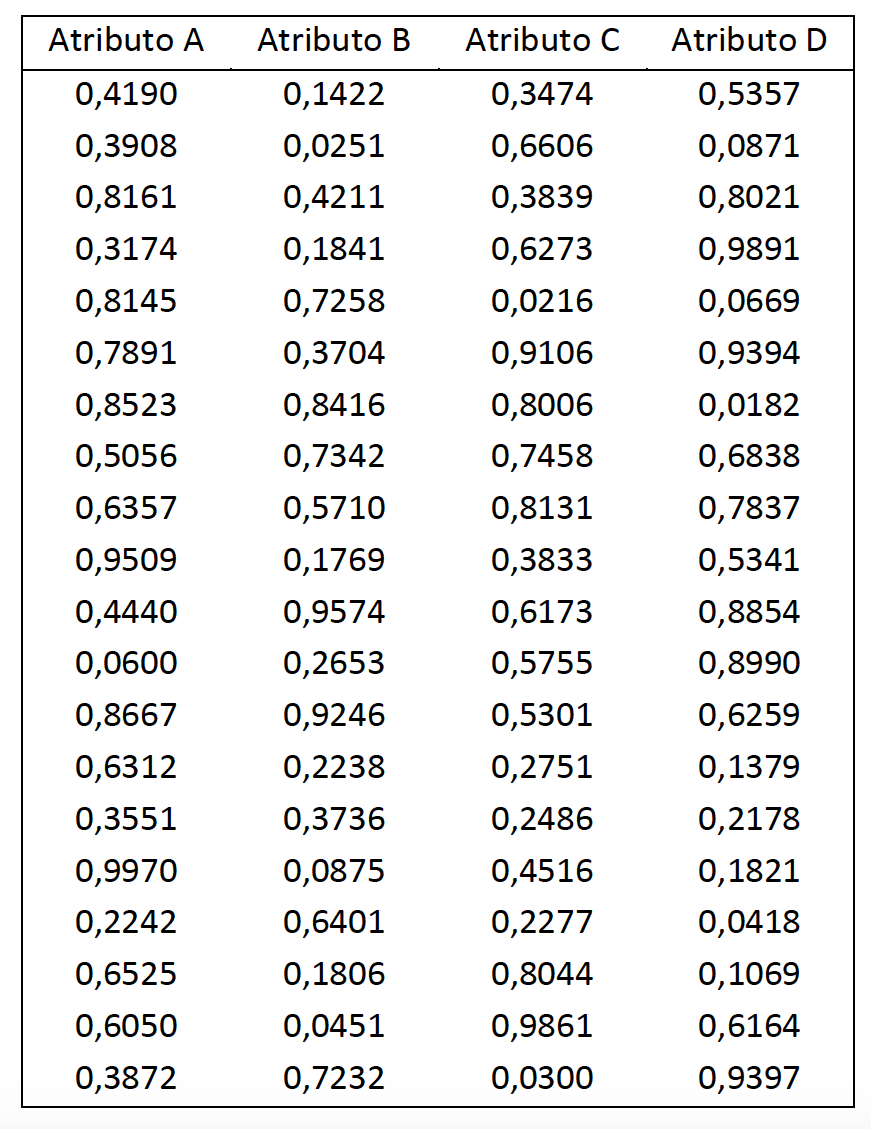
\includegraphics[width=5cm]{tabela.png} 
\end{figure}

\begin{enumerate}[label=\alph*]
  \item Calcule o domínio, a média e a mediana de cada atributo. \\
  \textit{Resposta:} 
    \begin{enumerate}[label=\alph*]
    \item \textbf{Média:} Atributo A = 0,5857 \\
      Atributo B = 0,4307 \\
      Atributo C = 0,5220 \\
      Atributo D = 0,5047
    \item \textbf{Mediana:} Atributo A = $\dfrac{0.605 + 0.6312}{2} = 0.6181$\\
    Atributo B = $\dfrac{0.3704 + 0.3736}{2} = 0.372$\\ 
    Atributo C = $\dfrac{0.5301 + 0.5755}{2} = 0.5528$\\ 
    Atributo D = $\dfrac{0.5357 + 0.6164}{2} = 0.5760$\\ 
    \end{enumerate}
  \item Calcule o primeiro, segundo e terceiro quartis para todos os atributos. \\
  \textit{Resposta:}
  \begin{enumerate}[label=\alph*]
    \item \textbf{Q1} \\
    Atributo A = 0.3872 \\
    Atributo B = 0.1769 \\
    Atributo C = 0.2751 \\
    Atributo D = 0.1069 
    \item \textbf{Q2} \\
    Atributo A = $\dfrac{0.605 + 0.6312}{2} = 0.6181$\\
    Atributo B = $\dfrac{0.3704 + 0.3736}{2} = 0.372$\\ 
    Atributo C = $\dfrac{0.5301 + 0.5755}{2} = 0.5528$\\ 
    Atributo D = $\dfrac{0.5357 + 0.6164}{2} = 0.5760$\\ 
    \item \textbf{Q3} \\
    Atributo A = 0.8161 \\
    Atributo B = 0.7258 \\
    Atributo C = 0.8006 \\
    Atributo D = 0.8854 
  \end{enumerate}
  \item  Desenhe o diagrama em caixa para todos os atributos. \\

  \textit{Resposta:}

  \begin{figure}[H]
    \centering 
    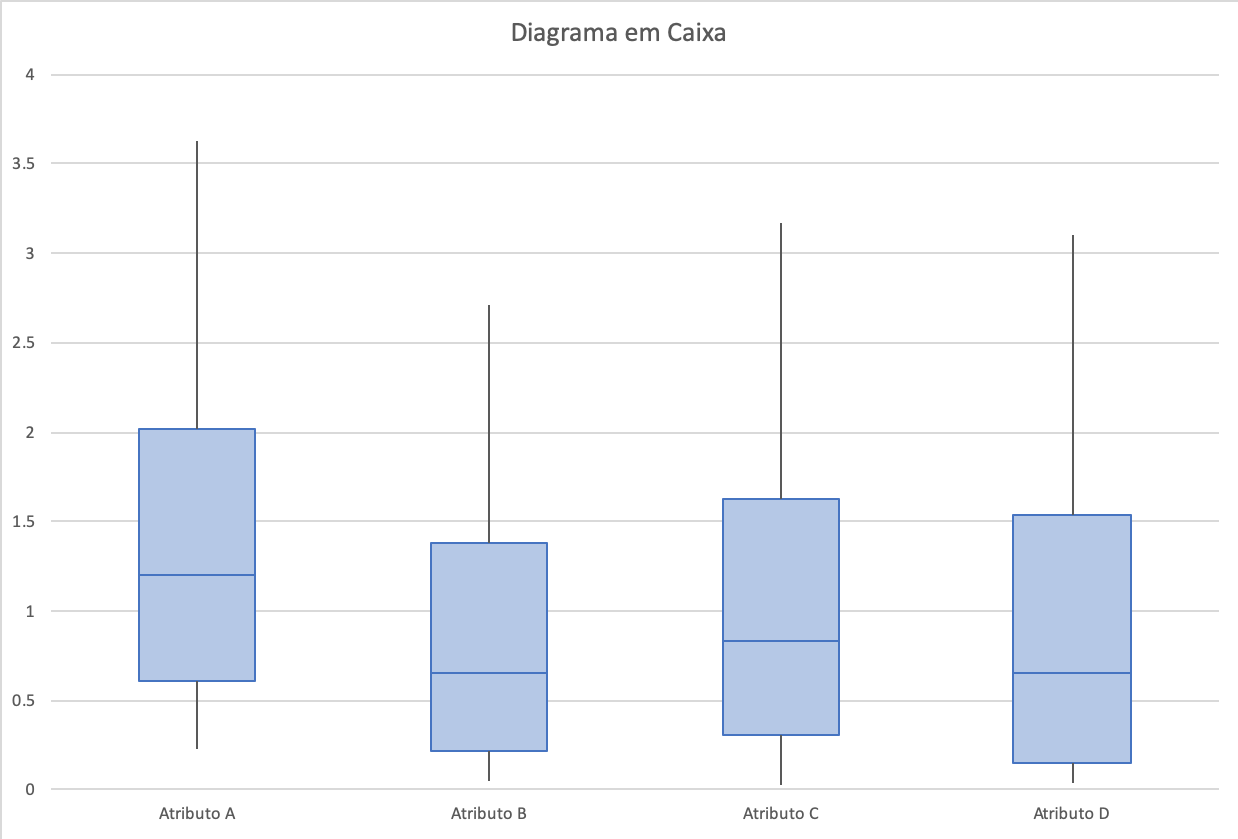
\includegraphics[width=14cm]{grafico_caixa.png} 
  \end{figure}
\end{enumerate}

\subsection{DESAFIO COMPUTACIONAL}
\subsubsection{O Capítulo 3 traz o exemplo do processo de análise descritiva de dados aplicado aos atributos Mês, Dia, DMC e DC da base Fires. Para este desafio, realize o mesmo processo para os atributos X, Y, Temp e UR da base Fires. Realize as etapas do processo de forma similar ao exemplo exposto no livro.}
\textit{Resposta:}

\end{document}